\section{Problems}
% !TeX spellcheck = en_GB

\begin{problem}{1}
Suppose that all link metrics in a graph has the same value. What
characterizes the paths found by a shortest--path algorithm?
\end{problem}

\begin{problem}{2}
Consider a situation where packets transmitted on a link will
either arrive without errors at the other end--point of the link,
or be lost. The probability of a packet loss on the link between
nodes $i$ and $j$ is denoted $P_{ij}$. Determine the function for
translating a link's packet loss rate into a metric, so that the
shortest paths are the paths that maximizes the probability that
the packets arrive at the destination, \ie determine $f()$ in the
relation: $C_{ij} = f(P_{ij})$.
\end{problem}

\begin{problem}{3}
Consider the graph in figure~\ref{fig:graphs2}. Determine the
shortest--paths from node A to all other nodes using the
Bellman--Ford algorithm. Repeat the problem with Dijkstra's
algorithm.
\begin{figure}[ht] \centering
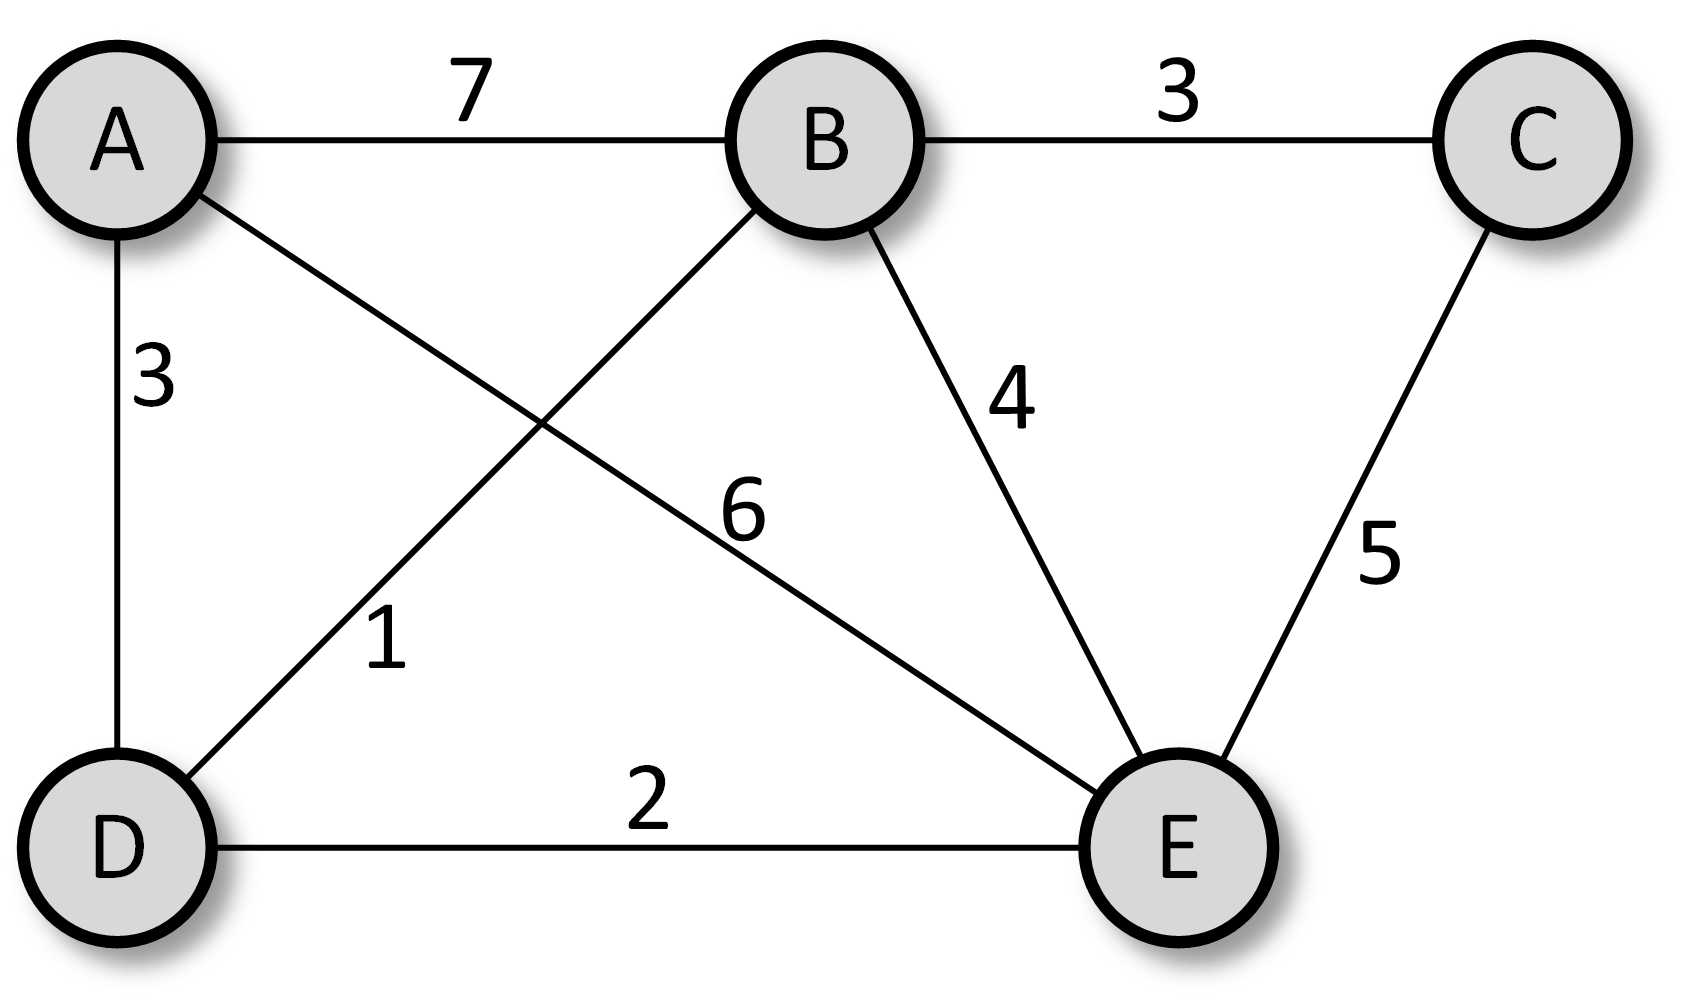
\includegraphics{graphs2.eps}
\caption{\label{fig:graphs2}Graph for problems 3}
\end{figure}
\end{problem}

\begin{problem}{4}
Explain how the Bellman--Ford algorithm can be modified to find
the shortest--paths to a destination node from all other nodes in
the graph.
\end{problem}
